\documentclass[11pt, oneside]{book}
\usepackage[pdftex,a4paper]{geometry}
\usepackage{pdfpages}
\usepackage{graphicx}
\usepackage{amssymb}
\usepackage{ifthen}
\usepackage{float}
\usepackage{calc}
\usepackage[export]{adjustbox}% http://ctan.org/pkg/adjustbox
\usepackage[scaled]{helvet}
\renewcommand\familydefault{\sfdefault} 
\usepackage[T1]{fontenc}
\pagestyle{empty}

\newcommand{\decal}[5]{
\begin{minipage}{\linewidth}
	\begin{minipage}[t]{0.3\textwidth}
       \vspace{0pt}
	\ifthenelse{\isodd{#1}}{
		\includegraphics[width=0.9\textwidth,page=#1,viewport=103 #3 291 #4,clip=true]{13GR_PistopioimeniSimansi_ISO_7010.pdf}
	}{
		\includegraphics[width=0.9\textwidth,page=#1,viewport=70 #3 261 #4,clip=true]{13GR_PistopioimeniSimansi_ISO_7010.pdf}
	}
	\end{minipage}
	\begin{minipage}[t]{0.6\textwidth}
\setlength{\parindent}{4em}
\setlength{\parskip}{1.2em}
       \vspace{0pt}\raggedright
	{\LARGE \textbf{#2}}
	
	
	#5
	\vspace{1cm}
	\end{minipage}
\end{minipage}
}
\newcommand{\action}[3]{\decal{#1}{#2}{520}{715}{#3}}
\newcommand{\prohib}[3]{\decal{#1}{#2}{495}{690}{#3}}
\newcommand{\warn}[3]{\decal{#1}{#2}{520}{715}{#3}}

\setlength{\parindent}{4em}
\setlength{\parskip}{1.5em}
\setlength{\textheight}{28cm}
\setlength{\textwidth}{19cm}
\setlength{\hoffset}{-2cm}
\setlength{\voffset}{-2cm}

\newcommand{\machinePage}[6]{%
\begin{center}
\vspace{0cm}
{\fontsize{50}{60} \textbf{#1}}

\action{49}{\textbf{#2}}{#3}
\begin{minipage}{\linewidth}
	\begin{minipage}[t]{0.5\textwidth}\vspace{0pt}#4\end{minipage}
	\begin{minipage}[t]{0.5\textwidth}\vspace{0pt}#5\end{minipage}
\end{minipage}
\vspace{0.2cm}

#6

If the machine is not clean or appears broken - then report this to the mailing list. Clean/fix prior to use.

\textbf{Report any damage, issues or accident within 24 hours to the mailing list.}
\end{center}
\pagebreak
}

\begin{document}

\machinePage{Large CNC Cutter}{Instructions Mandatory}{
	Instructions \textbf{prior} to use are mandatory. Check the wiki for whom can help you.

	Machine can only be used between 07:00 - 19:00 (be kind to our neighbours).
	
	Be very careful with viruses/media -- as we cannot re-install the software on the PC.
}{
\action{51}{Ear protection strongly recommended}{Note also that this machine should not be used after 19:00}
\action{52}{Eye protection recommended}{Especially when using very small cutters.}
\action{64}{Wear a mask when needed}{Especially when cutting materials such as MDF}
}{
\warn{124}{Machine can suddenly start}{%
	Machine can suddenly start moving; and can move under its own command (even when the PC is off).
	
	It will also start moving without warning when the PC is started/the software is started}
\warn{125}{Crushing}{Risk of crushing - the machine does not have any sensors that detect obstacles
This includes things such as your hands (do not lean on the blue rail) or tools you've left on the workspace.
}
}{
This machine contains commercial software which is locked to this specific hardware and OS install. Neither of which we can re-install (as we have no media and the suppliers have long gone out of business). So be very very careful with USB sticks and other media. A virus or malware may permanently kill this setup.
}

\machinePage{Abene Mill}{Instructions \& Approval Mandatory}{
	Instructions \textbf{prior} to use are mandatory. Check the wiki for whom can help you.

	Must have the `dangerous equipment waver' filed with the foundations trustees and been given approval or card access.	
}{
\prohib{100}{Do not wear gloves}{Especially strong leather ones. They get caught easily and then `help' ripping body parts off.}
\action{52}{Eye protection recommended}{Swarf will fly. Cutters can come loose. Broken cutters can fly very far and are razor sharp.}
\action{58}{Wear protective clothing}{Wear tight fitting clothing, keep long hair out tied up, no jewellery or anything else that can be caught by the machine.}
}{
\warn{125}{Crushing}{Risk of crushing - the machine does not have any sensors that detect obstacles.

Note that it can also run very slow; barely noticeable.}
\warn{117}{Slippery surface}{Floor will get very slippery; especially when using coolant.}
\warn{128}{Sharp rotating elements}{This machine is essentially a cutter without any guard whatsoever.}
}{
Only switch XYZ feeds when the machine is not running. Use the handwheel to get the gear fully locked in prior to starting the feed. Be sure to tighten all 4 nuts post rotating the head or all 4 nuts when moving the head laterally.

Try to avoid getting coolant or similar on the slide-ways - especially the Y slipway between machine and table. Use a shield or adjust the flow. Machine needs to be cleaned post use.  When using coolant - also empty the recess on the left of the table and clean out the t-Slots until dry.
}


\machinePage{Wood Lathe}{Instructions Mandatory}{
	Instructions \textbf{prior} to use are mandatory. Check the wiki for whom can help you.

	Must have the `dangerous equipment waver' filed with the foundations trustees and been given approval or card access.	
}{
\action{64}{Wear a mask when needed}{Especially when cutting materials such as MDF}
\action{58}{Wear protective clothing}{Wear tight fitting clothing, keep long hair out tied up, no jewellery or anything else that can be caught by the machine.}
}{
\action{52}{Eye protection mandatory}{}
\prohib{100}{Not recommended to wear gloves}{}
}{
}


%\action{49}{General mandatory action sign}
%\action{50}{Refer to instruction manual/booklet}
%\action{51}{Wear ear protection}
%\action{52}{Wear eye protection}
%\action{55}{Opaque eye protection must be worn}
%\action{57}{Wear protective gloves}
%\action{58}{Wear protective clothing}
%\action{64}{Wear a mask}
%\action{67}{Wear a welding mask}
%\action{74}{Use protective apron}
%\prohib{75}{General prohibition sign}
%\prohib{100}{Do not wear gloves}
%\warn{117}{Slippery surface}
%\warn{124}{Automatic start-up}
%\warn{125}{Crushing}
%\warn{128}{Sharp element}
%\warn{130}{Crushing of hands}


\end{document}  